\chapter{Crystals I: The Perfect Crystal and Metals}\label{ch:b1:crystals-metals}

A copper wire can be drawn thinner than a hair without breaking; a lump
of salt shatters under a hammer. A blacksmith heats a bar of iron until
it glows, hammers it, plunges it into water, and the bar comes out much
harder than it went in. The difference between these behaviours lies in
the way the atoms are stacked in the solid. Most solids are \omterm{def:b1:crystals-metals:crystal}{crystals}:
their atoms sit on a pattern that repeats itself, identical, billions of
times in every direction. This chapter describes such patterns, counts
their atoms, measures how tightly they are packed and where the gaps
between them lie, and uses the result to understand metals and alloys.
The next chapter applies the same tools to ionic, covalent and molecular
solids.

\begin{recall}
Metals lose their \omterm{def:b1:quantum-numbers:configuration}{valence electrons} easily: they have low ionisation
energies and electronegativities (\cref{ch:b1:periodicity}). Atomic radii
were defined in \cref{def:b1:periodicity:radius}. Density, a property
studied in physics, is used as known: $\rho = m/V$.
\end{recall}

\begin{omfigure}
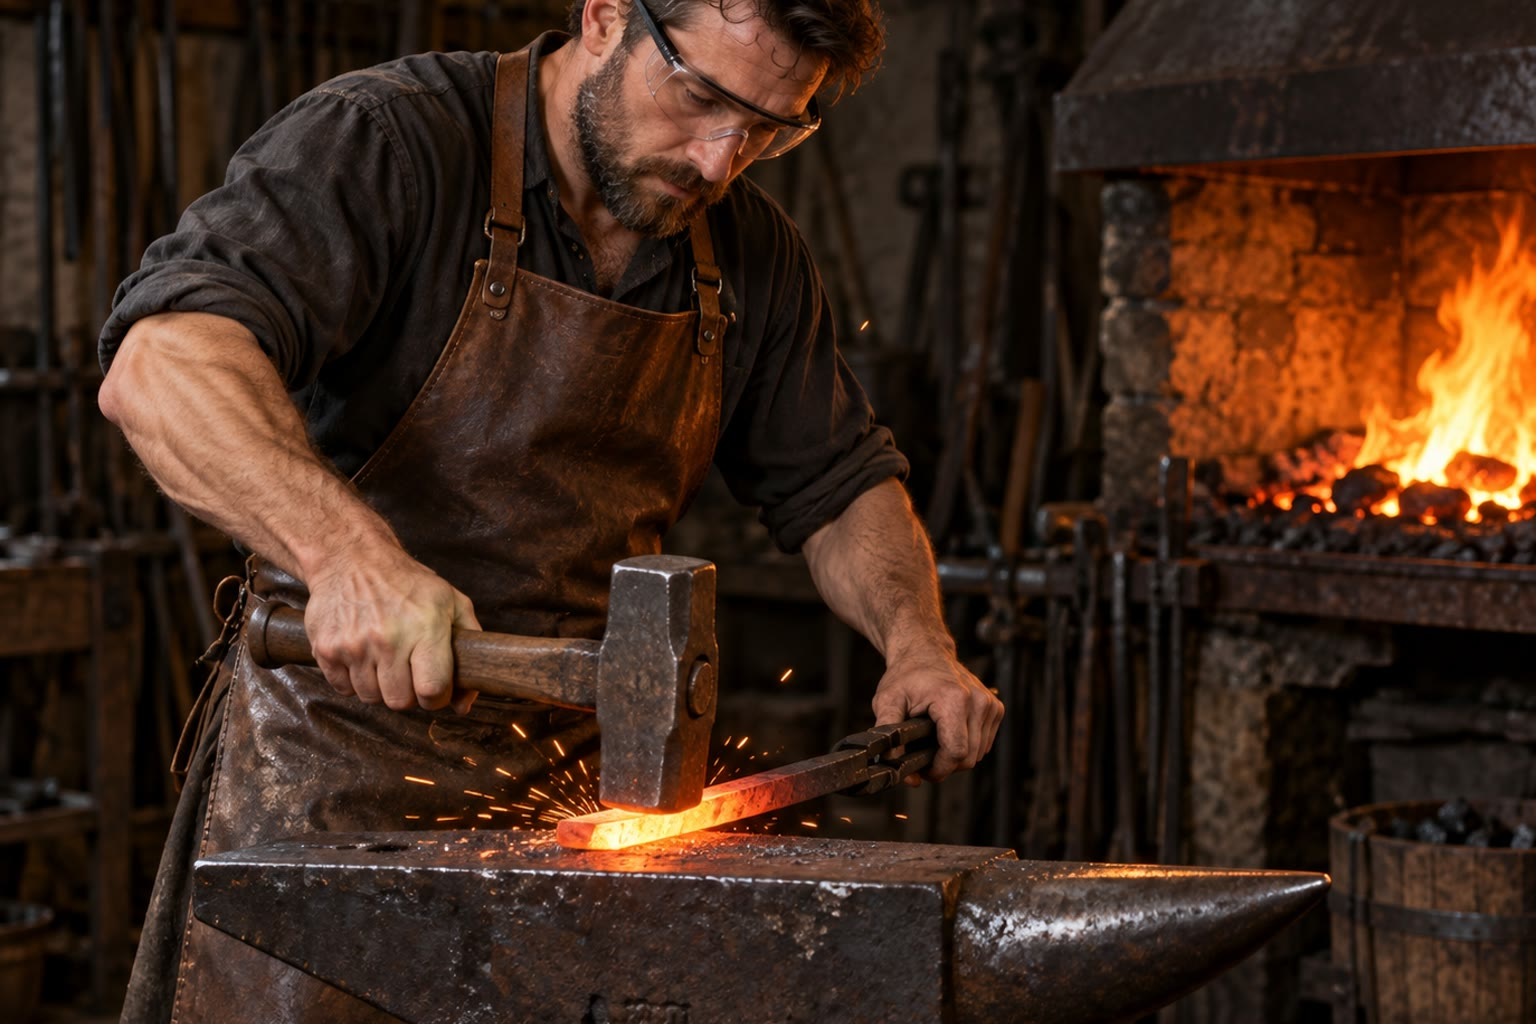
\includegraphics[width=0.55\linewidth]{images/book2/ai/b1-05-blacksmith.jpg}

{\small A blacksmith forging steel. Iron that glows orange has a
different \omterm{def:b1:crystals-metals:crystal}{crystal} structure from iron at room temperature, and can hold
more carbon (weekend problem).}
\end{omfigure}

\section{The perfect-crystal model}

\begin{definition}[Crystal, amorphous solid, perfect crystal]\label{def:b1:crystals-metals:crystal}
A \emph{crystal}\index{crystal} is a solid whose particles (atoms, ions
or molecules) are arranged in a pattern that repeats periodically in
three dimensions. A solid without such long-range order is an
\emph{amorphous solid}\index{amorphous solid} (glass, most plastics). The
\emph{perfect crystal model}\index{perfect crystal model} describes a
crystal as infinite and without defects: no missing or extra atoms, no
impurities, no boundaries.
\end{definition}

\begin{definition}[Lattice, motif, unit cell]\label{def:b1:crystals-metals:lattice}
A \emph{lattice}\index{lattice} is an infinite set of points, the
\emph{nodes}\index{node}, obtained from one of them by all the
translations $u\,\vec a + v\,\vec b + w\,\vec c$ with integer $u$, $v$,
$w$. The \omterm{def:b1:crystals-metals:crystal}{crystal} is obtained by placing on every node the same
\emph{motif}\index{motif} (one atom, a group of atoms or ions). A
\emph{unit cell}\index{unit cell} is a parallelepiped built on
$\vec a$, $\vec b$, $\vec c$ whose translations fill space; its edge
lengths and angles are the \emph{lattice parameters}\index{lattice parameters}
$a$, $b$, $c$, $\alpha$, $\beta$, $\gamma$. In a cubic cell
$a = b = c$ and the angles are $90^\circ$.
\end{definition}

\begin{remark}[Real crystals]\label{rem:b1:crystals-metals:real}
Real \omterm{def:b1:crystals-metals:crystal}{crystals} are finite and imperfect: they contain vacancies,
impurities, dislocations and grain boundaries, which govern many
properties (the ductility of copper, the hardness of steel). These
defects are studied in the Year 3 volume; the perfect \omterm{def:b1:crystals-metals:crystal}{crystal} gives the
geometry, density and \omterm{def:b1:crystals-metals:compactness}{compactness}, which defects barely change.
\end{remark}

\begin{definition}[Multiplicity of a cell]\label{def:b1:crystals-metals:multiplicity}
The \emph{multiplicity}\index{multiplicity} $Z$ of a cell is the number of
\omterm{def:b1:crystals-metals:lattice}{motifs} (or atoms) that belong to it, each atom shared with the
neighbouring cells counting for the fraction that lies inside it.
\end{definition}

\begin{method}[Counting the atoms of a cell]\label{met:b1:crystals-metals:count}
In a cubic cell an atom at a corner is shared by 8 cells and counts
$1/8$; on an edge it is shared by 4 and counts $1/4$; on a face it is
shared by 2 and counts $1/2$; inside it counts 1. Sum the contributions.
\end{method}

\begin{definition}[Coordination number]\label{def:b1:crystals-metals:coordination}
The \emph{coordination number}\index{coordination number} of a particle
in a solid is the number of its nearest neighbours, those at the
shortest distance.
\end{definition}

\begin{definition}[Compactness]\label{def:b1:crystals-metals:compactness}
The \emph{compactness}\index{compactness} (or packing fraction) of a
\omterm{def:b1:crystals-metals:crystal}{crystal} of hard spheres is the fraction of the volume occupied by the
spheres: for a cell of volume $V$ containing $Z$ spheres of radius $R$,
\[
  C = \frac{Z \cdot \frac43 \pi R^3}{V} .
\]
\end{definition}

\begin{proposition}[Density from the cell]\label{prop:b1:crystals-metals:density}
The density of a \omterm{def:b1:crystals-metals:crystal}{crystal} whose cell, of volume $V$, contains $Z$
particles of molar mass $M$ is
\[
  \rho = \frac{Z\,M}{N_A\,V} .
\]
\end{proposition}

\begin{proof}
The cell contains $Z$ particles, of mass $Z\,M/N_A$; the \omterm{def:b1:crystals-metals:crystal}{crystal} is
the cell repeated, so its density is that of one cell.
\end{proof}

\section{Close packings: face-centred cubic and hexagonal}

\begin{definition}[Close packing, FCC, HCP]\label{def:b1:crystals-metals:packings}
A \emph{close packing}\index{close packing} of identical spheres is built
from close-packed layers, in which each sphere touches six others, stacked
so that each sphere of a layer sits in a hollow of the layer below. The
stacking $ABCABC\dots$ gives the \emph{face-centred cubic}\index{face-centred cubic}
structure (FCC, or cubic close-packed); the stacking $ABAB\dots$
gives the \emph{hexagonal close-packed}\index{hexagonal close-packed}
structure (HCP). A third, non-close-packed, structure of metals is the
\emph{body-centred cubic}\index{body-centred cubic} structure (BCC), a
cube with one atom at each corner and one at its centre.
\end{definition}

\begin{omfigure}
\begin{tikzpicture}[font=\small]
  % layer A
  \foreach \i in {0,...,4} \foreach \j in {0,...,3} {
    \pgfmathsetmacro\x{\i+0.5*\j}
    \pgfmathsetmacro\y{0.866*\j}
    \draw[black!60, fill=omDef!25] (\x,\y) circle (0.5);
  }
  % layer B, in the hollows pointing up
  \foreach \i/\j in {1/0, 2/0, 3/0, 1/1, 2/1, 3/1, 1/2, 2/2} {
    \pgfmathsetmacro\x{\i+0.5*\j}
    \pgfmathsetmacro\y{0.866*\j+0.577}
    \draw[omThm!80!black, fill=omThm!25, fill opacity=0.75] (\x,\y) circle (0.5);
  }
  % C positions
  \foreach \i/\j in {1/0, 2/0, 3/0, 1/1, 2/1, 3/1} {
    \pgfmathsetmacro\x{\i+0.5+0.5*\j}
    \pgfmathsetmacro\y{0.866*\j+0.289}
    \fill[omMeth] (\x,\y) circle (0.11);
  }
  \node[anchor=west, align=left] at (6.6,1.6) {A: first layer (blue)\\B: second layer, in the\\\phantom{B: }hollows of A (red)\\C: the other hollows\\\phantom{C: }(green dots)};
\end{tikzpicture}

{\small Two close-packed layers seen from above. A third layer can sit
above the hollows marked C (stacking $ABC$, \omterm{def:b1:crystals-metals:packings}{face-centred cubic}) or above
the atoms of A (stacking $AB$, \omterm{def:b1:crystals-metals:packings}{hexagonal close-packed}).}
\end{omfigure}

\begin{proposition}[Face-centred cubic]\label{prop:b1:crystals-metals:fcc}
In the FCC structure the atoms occupy the eight corners and the six face
centres of a cube of edge $a$. Then $Z = 4$, the \omterm{def:b1:crystals-metals:coordination}{coordination number} is
12, the atoms touch along a face diagonal, $a\sqrt2 = 4R$, and the
\omterm{def:b1:crystals-metals:compactness}{compactness} is
\[
  C = \frac{\pi}{3\sqrt2} \approx 0.74 .
\]
\end{proposition}

\begin{proof}
$Z = 8 \times \frac18 + 6 \times \frac12 = 4$. A face-centre atom touches
the four corners of its face and the four face centres of each of the two
cells sharing the face: $4 + 4 + 4 = 12$ neighbours at $a\sqrt2/2$. On a
face diagonal, of length $a\sqrt2$, lie a corner atom, a face-centre atom
and a corner atom in contact: $a\sqrt2 = 4R$. Then
$C = 4 \cdot \frac43\pi R^3/a^3 = \frac{16}{3}\pi R^3/(2\sqrt2 R)^3 \cdot
\frac{1}{1} = \frac{16\pi}{3 \times 16\sqrt2} = \frac{\pi}{3\sqrt2}$.
\end{proof}

\begin{omfigure}
\tdplotsetmaincoords{60}{100}
\begin{tikzpicture}[tdplot_main_coords, font=\small]
  \pic {omcubeo={3}};
  \node[cellA=6mm] at (0,0,0) {};
  \node[cellA=6mm] at (0,3,0) {};
  \node[cellA=6mm, ball color=omDef!55] at (0,1.5,1.5) {};
  \node[cellA=6mm] at (0,0,3) {};
  \node[cellA=6mm, ball color=omDef!55] at (1.5,1.5,0) {};
  \node[cellA=6mm] at (0,3,3) {};
  \node[cellA=6mm, ball color=omDef!55] at (1.5,0,1.5) {};
  \node[cellA=6mm, ball color=omDef!55] at (1.5,3,1.5) {};
  \node[cellA=6mm] at (3,0,0) {};
  \node[cellA=6mm, ball color=omDef!55] at (1.5,1.5,3) {};
  \node[cellA=6mm] at (3,3,0) {};
  \node[cellA=6mm, ball color=omDef!55] at (3,1.5,1.5) {};
  \node[cellA=6mm] at (3,0,3) {};
  \node[cellA=6mm] at (3,3,3) {};
  \draw[omThm, thick] (3,0,0) -- (3,3,3);
\end{tikzpicture}
\hspace{1.2cm}
\begin{tikzpicture}[tdplot_main_coords, font=\small]
  \pic {omcubeo={3}};
  \node[cellA=7mm] at (0,0,0) {};
  \node[cellA=7mm] at (0,3,0) {};
  \node[cellA=7mm] at (0,0,3) {};
  \node[cellA=7mm] at (0,3,3) {};
  \node[cellA=7mm, ball color=omDef!55] at (1.5,1.5,1.5) {};
  \node[cellA=7mm] at (3,0,0) {};
  \node[cellA=7mm] at (3,3,0) {};
  \node[cellA=7mm] at (3,0,3) {};
  \node[cellA=7mm] at (3,3,3) {};
  \draw[omThm, thick] (3,0,0) -- (0,3,3);
\end{tikzpicture}

{\small Left: the \omterm{def:b1:crystals-metals:packings}{face-centred cubic} cell (corner atoms grey, face-centre
atoms blue). The atoms touch along a face diagonal (red line,
$a\sqrt2 = 4R$). Right: the \omterm{def:b1:crystals-metals:packings}{body-centred cubic} cell; the atoms touch along
the main diagonal (red line, $a\sqrt3 = 4R$).
Atoms drawn smaller than their contact size, for clarity.}
\end{omfigure}

\begin{proposition}[Hexagonal close-packed]\label{prop:b1:crystals-metals:hcp}
In the HCP structure the conventional hexagonal prism, of base edge $a$
and height $c$, contains 6 atoms; the \omterm{def:b1:crystals-metals:coordination}{coordination number} is 12; for
touching spheres $a = 2R$, $c/a = \sqrt{8/3} \approx 1.633$, and the
\omterm{def:b1:crystals-metals:compactness}{compactness} is the same as for FCC, $\pi/(3\sqrt2) \approx 0.74$.
\end{proposition}

\begin{proof}
The prism has 12 corner atoms shared by 6 prisms, 2 face-centre atoms
shared by 2, and 3 atoms inside: $12/6 + 2/2 + 3 = 6$. Each atom touches
six neighbours in its layer and three in each adjacent layer: 12. An atom
of layer B sits on three touching atoms of layer A, forming a regular
tetrahedron of edge $2R$, whose height is $2R\sqrt{2/3}$; two layers
apart, $c = 4R\sqrt{2/3}$, so $c/a = 2\sqrt{2/3} = \sqrt{8/3}$. The prism
volume is $\frac{3\sqrt3}{2}a^2 c = \frac{3\sqrt3}{2}(2R)^2 \cdot
4R\sqrt{2/3} = 24\sqrt2\,R^3$, and $C = 6 \cdot \frac43\pi R^3/(24\sqrt2
R^3) = \pi/(3\sqrt2)$.
\end{proof}

\begin{omfigure}
\tdplotsetmaincoords{70}{113}
\begin{tikzpicture}[tdplot_main_coords, font=\small, scale=1.25]
  \pic[transform shape] {omhexprismo={1.6}{2.6}};
  \node[cellA=6mm] at (-1.6,0,0) {};
  \node[cellA=6mm] at (-0.8,-1.386,0) {};
  \node[cellA=6mm] at (-1.6,0,2.6) {};
  \node[cellA=6mm] at (-0.8,-1.386,2.6) {};
  \node[cellA=6mm] at (-0.8,1.386,0) {};
  \node[cellA=6mm, ball color=omThm!60] at (-0.8,0.462,1.3) {};
  \node[cellA=6mm] at (0,0,0) {};
  \node[cellA=6mm, ball color=omThm!60] at (0,-0.924,1.3) {};
  \node[cellA=6mm] at (0.8,-1.386,0) {};
  \node[cellA=6mm] at (-0.8,1.386,2.6) {};
  \node[cellA=6mm] at (0,0,2.6) {};
  \node[cellA=6mm] at (0.8,-1.386,2.6) {};
  \node[cellA=6mm] at (0.8,1.386,0) {};
  \node[cellA=6mm, ball color=omThm!60] at (0.8,0.462,1.3) {};
  \node[cellA=6mm] at (1.6,0,0) {};
  \node[cellA=6mm] at (0.8,1.386,2.6) {};
  \node[cellA=6mm] at (1.6,0,2.6) {};
\end{tikzpicture}

{\small The \omterm{def:b1:crystals-metals:packings}{hexagonal close-packed} prism, of base edge $a$ (the side of
the hexagon) and height $c$: layers A (grey) at the bottom and the top,
layer B (red) half-way, sitting in the hollows of A.}
\end{omfigure}

\section{Body-centred cubic and the metallic elements}

\begin{proposition}[Body-centred cubic]\label{prop:b1:crystals-metals:bcc}
In the BCC structure $Z = 2$, the \omterm{def:b1:crystals-metals:coordination}{coordination number} is 8, the atoms
touch along the main diagonal of the cube, $a\sqrt3 = 4R$, and the
\omterm{def:b1:crystals-metals:compactness}{compactness} is
\[
  C = \frac{\pi\sqrt3}{8} \approx 0.68 .
\]
\end{proposition}

\begin{proof}
$Z = 8 \times \frac18 + 1 = 2$. The central atom touches the eight
corners: the main diagonal $a\sqrt3$ holds a corner, the centre and a
corner, $a\sqrt3 = 4R$. Then $C = 2 \cdot \frac43\pi R^3/a^3 =
\frac83\pi R^3 (\sqrt3/(4R))^3 = \frac83\pi \cdot \frac{3\sqrt3}{64} =
\frac{\pi\sqrt3}{8}$.
\end{proof}

\begin{proposition}[Close packing is the densest]\label{prop:b1:crystals-metals:kepler}
No packing of identical spheres has a \omterm{def:b1:crystals-metals:compactness}{compactness} larger than
$\pi/(3\sqrt2) \approx 0.7405$, the value of FCC and HCP.
\end{proposition}
\admitted

\begin{history}[Kepler's conjecture, 1611--2017]
In a short essay on snowflakes, written in 1611, Johannes Kepler stated
that no way of stacking cannonballs could be denser than the grocer's
pyramid, the \omterm{def:b1:crystals-metals:packings}{face-centred cubic} packing. The statement resisted proof for
almost four centuries. Thomas Hales gave a computer-assisted proof in
1998, and a formal proof checked line by line by computer was completed in
2014 and published in 2017.
\end{history}

\begin{example}[Three metals]\label{ex:b1:crystals-metals:metals}
Copper is FCC with $a = \qty{361.5}{pm}$: $R = a\sqrt2/4 =
\qty{127.8}{pm}$ and $\rho = 4 \times 63.55/(6.022 \times 10^{23} \times
(3.615 \times 10^{-8})^3) = \qty{8.93}{g/cm^3}$, the measured density.
Iron at room temperature ($\alpha$-iron) is BCC with $a = \qty{286.7}{pm}$:
$R = \qty{124.1}{pm}$, $\rho = \qty{7.87}{g/cm^3}$. Magnesium is HCP with
$a = \qty{320.9}{pm}$ and $c = \qty{521.0}{pm}$: $c/a = 1.624$, close to
the ideal $1.633$; zinc, with $c/a = 1.856$, is an elongated hexagonal
packing.
% ledger: lat:Cu, rho:Cu, lat:Fe-alpha, rho:Fe, lat:Mg.a, lat:Mg.c,
% lat:Zn.a, lat:Zn.c, aw:Cu, aw:Fe, const:NA
\end{example}

\begin{center}
\small
\begin{tabular}{lllccc}
\hline
metal & structure & $a$ (pm) & $R$ (pm) & $\rho$ computed & $\rho$ measured \\
\hline
aluminium & FCC & 405.0 & 143.2 & 2.70 & 2.70 \\
copper & FCC & 361.5 & 127.8 & 8.93 & 8.93 \\
silver & FCC & 408.6 & 144.5 & 10.50 & 10.50 \\
sodium & BCC & 429.1 & 185.8 & 0.967 & 0.97 \\
$\alpha$-iron & BCC & 286.7 & 124.1 & 7.87 & 7.87 \\
tungsten & BCC & 316.5 & 137.0 & 19.26 & 19.3 \\
\hline
\end{tabular}
\end{center}
% ledger: lat:Al, lat:Cu, lat:Ag, lat:Na, lat:Fe-alpha, lat:W, rho:Al,
% rho:Cu, rho:Ag, rho:Na, rho:Fe, rho:W (densities in g/cm3)

\begin{omfigure}
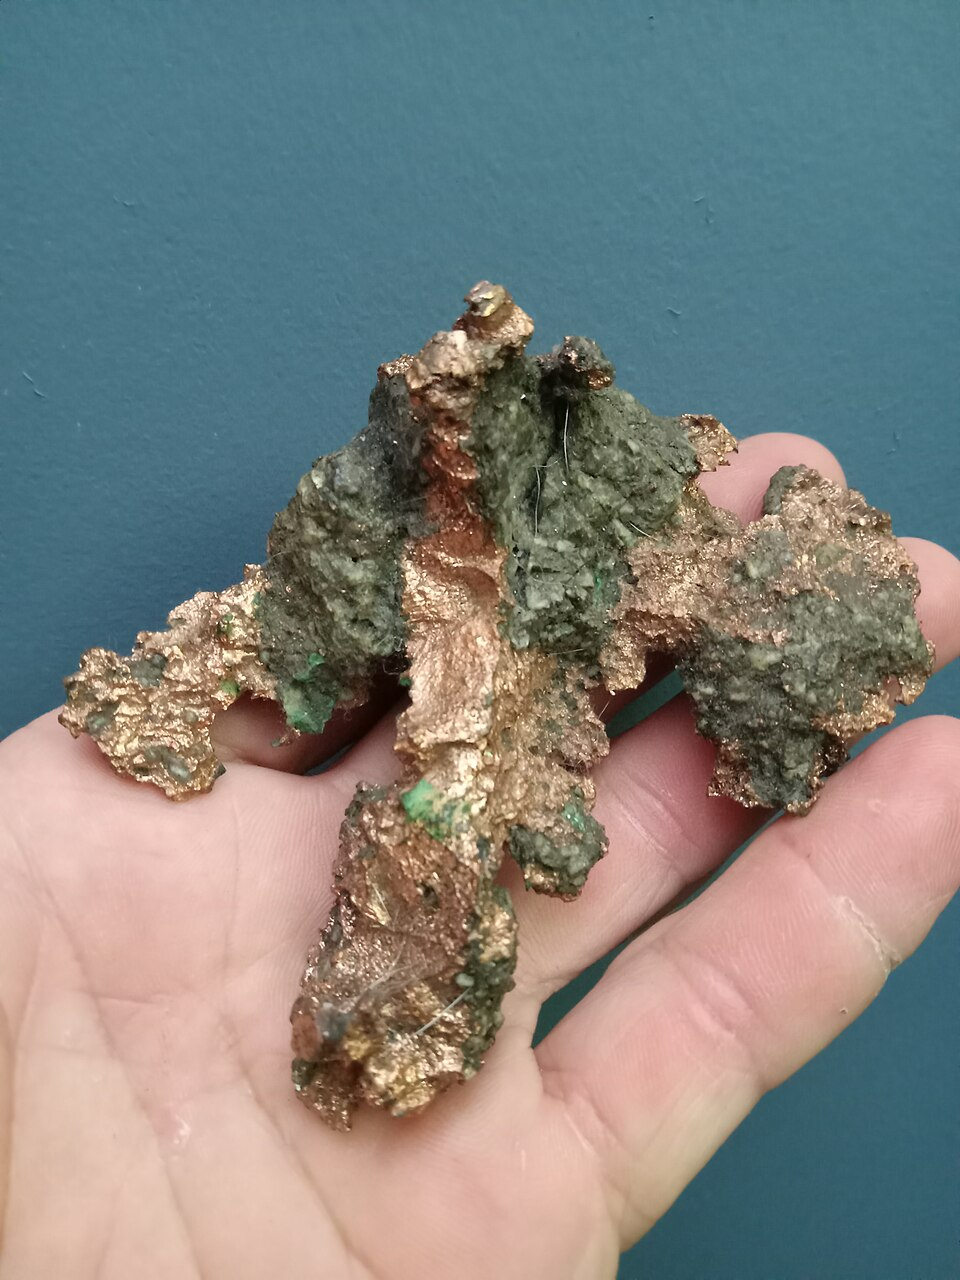
\includegraphics[width=0.36\linewidth]{images/book2/native-copper.jpg}

{\small A specimen of native copper. Its branching shapes grew as
\omterm{def:b1:crystals-metals:crystal}{crystals}; the metal underneath is a mosaic of FCC grains.
Photo: CC0 (Wikimedia Commons).}
\end{omfigure}

\section{Interstitial sites}

\begin{definition}[Interstitial sites]\label{def:b1:crystals-metals:site}
An \emph{interstitial site}\index{interstitial site} is a gap between the
atoms of a \omterm{def:b1:crystals-metals:crystal}{crystal} where a smaller atom can sit. A \emph{tetrahedral
site}\index{tetrahedral site} lies at the centre of a tetrahedron of four
atoms, an \emph{octahedral site}\index{octahedral site} at the centre of
an octahedron of six. The \emph{habitability}\index{habitability} of a
site is the radius of the largest sphere that fits in it without pushing
the surrounding atoms apart.
\end{definition}

\begin{proposition}[Sites of the FCC structure]\label{prop:b1:crystals-metals:sites}
An FCC cell contains 4 \omterm{def:b1:crystals-metals:site}{octahedral sites}, at the centre of the cube and at
the middles of its 12 edges, and 8 \omterm{def:b1:crystals-metals:site}{tetrahedral sites}, at the centres of
the 8 small cubes of edge $a/2$. For touching atoms of radius $R$, the
habitabilities are
\[
  r_O = (\sqrt2 - 1)R \approx 0.414\,R, \qquad
  r_T = \left(\sqrt{\tfrac32} - 1\right)R \approx 0.225\,R .
\]
\end{proposition}

\begin{proof}
\omterm{def:b1:crystals-metals:site}{Octahedral sites}: $1 + 12 \times \frac14 = 4$, as many as atoms. The
centre of the cube is $a/2$ from the six face centres: $r_O + R = a/2$
with $a = 2\sqrt2 R$, so $r_O = (\sqrt2 - 1)R$. \omterm{def:b1:crystals-metals:site}{Tetrahedral sites}: the
centre of a small cube of edge $a/2$ is half its main diagonal,
$\frac{a}{2}\cdot\frac{\sqrt3}{2} = \frac{a\sqrt3}{4}$, from the four atoms
at alternate corners: $r_T + R = \frac{\sqrt3}{4}\,2\sqrt2\,R =
\sqrt{\tfrac32}\,R$.
\end{proof}

\begin{omfigure}
\tdplotsetmaincoords{60}{100}
\begin{tikzpicture}[tdplot_main_coords, font=\small]
  \pic {omcubeo={3}};
  \node[cellA=3.6mm] at (0,0,0) {};
  \node[cellsite=4mm, draw=omThm, fill=omThm!30] at (0,1.5,0) {};
  \node[cellA=3.6mm] at (0,3,0) {};
  \node[cellsite=4mm, draw=omThm, fill=omThm!30] at (0,0,1.5) {};
  \node[cellA=3.6mm] at (0,1.5,1.5) {};
  \node[cellsite=4mm, draw=omThm, fill=omThm!30] at (0,3,1.5) {};
  \node[cellsite=4mm, draw=omThm, fill=omThm!30] at (1.5,0,0) {};
  \node[cellA=3.6mm] at (0,0,3) {};
  \node[cellA=3.6mm] at (1.5,1.5,0) {};
  \node[cellsite=4mm, draw=omThm, fill=omThm!30] at (0,1.5,3) {};
  \node[cellsite=4mm, draw=omThm, fill=omThm!30] at (1.5,3,0) {};
  \node[cellA=3.6mm] at (0,3,3) {};
  \node[cellA=3.6mm] at (1.5,0,1.5) {};
  \node[cellsite=5mm, draw=omThm, fill=omThm!30] at (1.5,1.5,1.5) {};
  \node[cellA=3.6mm] at (1.5,3,1.5) {};
  \node[cellA=3.6mm] at (3,0,0) {};
  \node[cellsite=4mm, draw=omThm, fill=omThm!30] at (1.5,0,3) {};
  \node[cellsite=4mm, draw=omThm, fill=omThm!30] at (3,1.5,0) {};
  \node[cellA=3.6mm] at (1.5,1.5,3) {};
  \node[cellA=3.6mm] at (3,3,0) {};
  \node[cellsite=4mm, draw=omThm, fill=omThm!30] at (1.5,3,3) {};
  \node[cellsite=4mm, draw=omThm, fill=omThm!30] at (3,0,1.5) {};
  \node[cellA=3.6mm] at (3,1.5,1.5) {};
  \node[cellsite=4mm, draw=omThm, fill=omThm!30] at (3,3,1.5) {};
  \node[cellA=3.6mm] at (3,0,3) {};
  \node[cellsite=4mm, draw=omThm, fill=omThm!30] at (3,1.5,3) {};
  \node[cellA=3.6mm] at (3,3,3) {};
  \node[below] at (1.5,1.5,-1.5) {octahedral sites (red)};
\end{tikzpicture}
\hspace{1.2cm}
\begin{tikzpicture}[tdplot_main_coords, font=\small]
  \pic {omcubeo={3}};
  \node[cellA=3.6mm] at (0,0,0) {};
  \node[cellA=3.6mm] at (0,3,0) {};
  \node[cellA=3.6mm] at (0,1.5,1.5) {};
  \node[cellsite=4mm, fill=omDef!30] at (0.75,0.75,0.75) {};
  \node[cellsite=4mm, fill=omDef!30] at (0.75,2.25,0.75) {};
  \node[cellA=3.6mm] at (0,0,3) {};
  \node[cellA=3.6mm] at (1.5,1.5,0) {};
  \node[cellsite=4mm, fill=omDef!30] at (0.75,0.75,2.25) {};
  \node[cellA=3.6mm] at (0,3,3) {};
  \node[cellA=3.6mm] at (1.5,0,1.5) {};
  \node[cellsite=4mm, fill=omDef!30] at (0.75,2.25,2.25) {};
  \node[cellsite=4mm, fill=omDef!30] at (2.25,0.75,0.75) {};
  \node[cellA=3.6mm] at (1.5,3,1.5) {};
  \node[cellA=3.6mm] at (3,0,0) {};
  \node[cellsite=4mm, fill=omDef!30] at (2.25,2.25,0.75) {};
  \node[cellA=3.6mm] at (1.5,1.5,3) {};
  \node[cellA=3.6mm] at (3,3,0) {};
  \node[cellsite=4mm, fill=omDef!30] at (2.25,0.75,2.25) {};
  \node[cellsite=4mm, fill=omDef!30] at (2.25,2.25,2.25) {};
  \node[cellA=3.6mm] at (3,1.5,1.5) {};
  \node[cellA=3.6mm] at (3,0,3) {};
  \node[cellA=3.6mm] at (3,3,3) {};
  \draw[omDef!70!black, thin] (0,0,0) -- (0.75,0.75,0.75) -- (1.5,1.5,0)
    (0.75,0.75,0.75) -- (1.5,0,1.5) (0.75,0.75,0.75) -- (0,1.5,1.5);
  \node[below] at (1.5,1.5,-1.5) {tetrahedral sites (blue)};
\end{tikzpicture}

{\small \omterm{def:b1:crystals-metals:site}{Interstitial sites} of the FCC cell. Left: the \omterm{def:b1:crystals-metals:site}{octahedral site} at
the centre and those at the edge middles (shared by four cells). Right:
the eight \omterm{def:b1:crystals-metals:site}{tetrahedral sites} at the centres of the eighths of the cube,
one shown joined to its four atoms.}
\end{omfigure}

\section{Metallic bonding and alloys}

\begin{definition}[Metallic bond]\label{def:b1:crystals-metals:metallic-bond}
In the \emph{metallic bond}\index{metallic bond}, each atom of a metal
gives its \omterm{def:b1:quantum-numbers:configuration}{valence electrons} to the whole \omterm{def:b1:crystals-metals:crystal}{crystal}: the solid is a \omterm{def:b1:crystals-metals:lattice}{lattice}
of cations bathed in electrons that belong to no atom in particular and
move freely through it. The bond is the attraction between the cations
and this shared electron cloud; it is not directed.
\end{definition}

\begin{proposition}[Properties of metals]\label{prop:b1:crystals-metals:properties}
The \omterm{def:b1:crystals-metals:metallic-bond}{metallic bond} explains the properties of metals: the mobile electrons
conduct electricity and heat and reflect light (lustre); because the bond
is not directed, layers of atoms can slide over one another without
breaking the \omterm{def:b1:crystals-metals:crystal}{crystal} (ductility, malleability), and \omterm{def:b1:crystals-metals:packings}{close packings}, which
maximise the number of neighbours, are the most common structures.
\end{proposition}
\admitted

\begin{definition}[Alloys]\label{def:b1:crystals-metals:alloy}
An alloy is a metallic solid made of several elements. In a
\emph{substitutional alloy}\index{substitutional alloy} the atoms of the
added element replace atoms of the host on its \omterm{def:b1:crystals-metals:lattice}{lattice}; this requires
radii within about 15\,\% of each other (copper and nickel, copper and
zinc in brass). In an \emph{interstitial alloy}\index{interstitial alloy}
small atoms (\ce{H}, \ce{C}, \ce{N}, \ce{B}) occupy \omterm{def:b1:crystals-metals:site}{interstitial sites} of
the host (carbon in steel).
\end{definition}

\begin{definition}[Allotropy]\label{def:b1:crystals-metals:allotropy}
Different \omterm{def:b1:crystals-metals:crystal}{crystal} structures of the same element are its
\emph{allotropes}\index{allotrope}. Iron is BCC ($\alpha$-iron) at room
temperature; it has been measured FCC ($\gamma$-iron) from \qty{1189}{K}
to \qty{1661}{K}, and BCC again ($\delta$-iron) at \qty{1662}{K}, up to
its melting point. Carbon exists as diamond and as graphite
(\cref{ch:b1:crystals-ionic-covalent}).
% ledger: lat:Fe-alpha, lat:Fe-gamma-1189, lat:Fe-gamma-1661,
% lat:Fe-delta-1662
\end{definition}

\begin{example}[Steel]\label{ex:b1:crystals-metals:steel}
Carbon, of \omterm{def:b1:periodicity:radius}{covalent radius} \qty{77}{pm} (half the \ce{C-C} distance in
diamond), is too large for the sites of iron without distortion, but much
less so in $\gamma$-iron, whose \omterm{def:b1:crystals-metals:site}{octahedral sites} are the largest. Steel
is made by dissolving carbon in hot $\gamma$-iron; quenched, the carbon is
trapped as the iron returns to a body-centred structure, which it
distorts, and the distorted \omterm{def:b1:crystals-metals:crystal}{crystal} is hard.
% ledger: lat:C-diamond (r = a sqrt3 / 8 = 77.2 pm)
\end{example}

\begin{remark}[The iron transitions]\label{rem:b1:crystals-metals:iron-T}
The temperatures of \cref{def:b1:crystals-metals:allotropy} are those of
pure iron at atmospheric pressure; dissolved carbon lowers the
temperature at which $\gamma$-iron forms, which makes steel workable.
Phase diagrams of alloys are studied in the Year 2 volume.
\end{remark}

\section{Exercises}

\begin{exercise}[$\star$]\label{exo:b1:crystals-metals:1}
Count the atoms of a simple cubic cell (atoms at the corners only), of a
BCC cell and of an FCC cell, and give the \omterm{def:b1:crystals-metals:coordination}{coordination number} in each.
\end{exercise}

\begin{exercise}[$\star$]\label{exo:b1:crystals-metals:2}
Show that the \omterm{def:b1:crystals-metals:compactness}{compactness} of the simple cubic structure (atoms touching
along an edge) is $\pi/6$, and compare with FCC and BCC.
\end{exercise}

\begin{exercise}[$\star$]\label{exo:b1:crystals-metals:3}
Aluminium is FCC with $a = \qty{405.0}{pm}$. Compute its atomic radius and
its density ($M = \qty{26.98}{g/mol}$).
% ledger: lat:Al, aw:Al
\end{exercise}

\begin{exercise}[$\star$]\label{exo:b1:crystals-metals:4}
Sodium is BCC with $a = \qty{429.1}{pm}$. Compute its atomic radius and
its density ($M = \qty{22.99}{g/mol}$), and compare with the measured
\qty{0.97}{g/cm^3}.
% ledger: lat:Na, rho:Na, aw:Na
\end{exercise}

\begin{exercise}[$\star\star$]\label{exo:b1:crystals-metals:5}
Silver is FCC and its density is \qty{10.50}{g/cm^3}
($M = \qty{107.87}{g/mol}$). Compute the \omterm{def:b1:crystals-metals:lattice}{lattice} parameter and the atomic
radius.
% ledger: rho:Ag, aw:Ag
\end{exercise}

\begin{exercise}[$\star\star$]\label{exo:b1:crystals-metals:6}
Show that in an HCP structure of touching spheres $c/a = \sqrt{8/3}$.
Magnesium has $a = \qty{320.9}{pm}$, $c = \qty{521.0}{pm}$. Compute $c/a$
and the density of magnesium ($M = \qty{24.31}{g/mol}$).
% ledger: lat:Mg.a, lat:Mg.c, aw:Mg
\end{exercise}

\begin{exercise}[$\star\star$]\label{exo:b1:crystals-metals:7}
In an FCC cell of edge $a$, give the coordinates of the 4 atoms that
belong to the cell, of the 4 \omterm{def:b1:crystals-metals:site}{octahedral sites} and of the 8 \omterm{def:b1:crystals-metals:site}{tetrahedral
sites}. How many of each per atom?
\end{exercise}

\begin{exercise}[$\star\star$]\label{exo:b1:crystals-metals:8}
Copper and nickel are both FCC, with $a = \qty{361.5}{pm}$ and
$a = \qty{352.4}{pm}$. Compute their atomic radii. They form a
\omterm{def:b1:crystals-metals:alloy}{substitutional alloy} in all proportions: explain. What kind of alloy can
hydrogen, a very small atom, form with a metal?
% ledger: lat:Cu, lat:Ni
\end{exercise}

\begin{exercise}[$\star\star$]\label{exo:b1:crystals-metals:9}
Tungsten is BCC with $a = \qty{316.5}{pm}$. Compute its radius, its
density ($M = \qty{183.84}{g/mol}$) and the number of atoms in
\qty{1}{cm^3}.
% ledger: lat:W, aw:W
\end{exercise}

\begin{exercise}[$\star\star\star$]\label{exo:b1:crystals-metals:10}
In the BCC structure, an \omterm{def:b1:crystals-metals:site}{octahedral site} lies at the centre of each face
(and at the middle of each edge), and a \omterm{def:b1:crystals-metals:site}{tetrahedral site} at
$(\frac{a}{2}, \frac{a}{4}, 0)$ on each face. Show that their
habitabilities are $r_O = \frac{2 - \sqrt3}{4}\,a$ and
$r_T = \frac{\sqrt5 - \sqrt3}{4}\,a$, and express them as fractions of
$R$. Which site is larger?
\end{exercise}

\begin{exercise}[$\star\star\star$]\label{exo:b1:crystals-metals:11}
A metal crystallises with $Z$ atoms per cubic cell of edge $a$. Show that
the \omterm{def:b1:crystals-metals:compactness}{compactness} can be written $C = \frac{4\pi R^3 Z}{3a^3}$, then that
$C = \frac{\pi\rho N_A}{6M}\,(2R)^3$. Apply to copper ($R = \qty{127.8}{pm}$,
$\rho = \qty{8.93}{g/cm^3}$) to check the value $0.74$.
\end{exercise}

\begin{exercise}[$\star\star\star$]\label{exo:b1:crystals-metals:12}
Gold is FCC with $a = \qty{407.8}{pm}$ and silver FCC with
$a = \qty{408.6}{pm}$. Gold and silver mix in all proportions. Estimate the
\omterm{def:b1:crystals-metals:lattice}{lattice} parameter of an alloy with 50\,\% atoms of each (assume the
average) and its density ($M(\ce{Au}) = \qty{196.97}{g/mol}$,
$M(\ce{Ag}) = \qty{107.87}{g/mol}$).
% ledger: lat:Au, lat:Ag, aw:Au, aw:Ag
\end{exercise}

\section{Problem: Why Steel Holds Carbon}

\begin{problem}[{Weekend problem --- iron below and above its transition
near 1190\,K, the holes between its atoms, and the room they leave for
carbon}]
\label{pb:b1:crystals-metals:1}
Data: $M(\ce{Fe}) = \qty{55.845}{g/mol}$, $M(\ce{C}) = \qty{12.011}{g/mol}$,
$N_A = \qty{6.022e23}{mol^{-1}}$. At room temperature $\alpha$-iron is BCC
with $a = \qty{286.65}{pm}$. At \qty{1189}{K}, just above the transition,
$\alpha$-iron (still present below the transition) is measured with
$a = \qty{289.8}{pm}$ and $\gamma$-iron, FCC, with $a = \qty{363.9}{pm}$.
Diamond is cubic with $a = \qty{356.68}{pm}$, each carbon touching four
others at a quarter of the main diagonal.
% ledger: lat:Fe-alpha, lat:Fe-alpha-1189, lat:Fe-gamma-1189,
% lat:C-diamond, aw:Fe, aw:C, const:NA

\medskip
\noindent\textbf{Part I --- $\alpha$-iron at room temperature.}
\begin{enumerate}
  \item How many atoms belong to a BCC cell? What is the \omterm{def:b1:crystals-metals:coordination}{coordination
        number}?
  \item Along which line do the atoms touch? Compute the radius of an
        iron atom.
  \item Compute the density of $\alpha$-iron.
  \item How many iron atoms are there in \qty{1}{cm^3} of $\alpha$-iron?
  \item Compute the \omterm{def:b1:crystals-metals:compactness}{compactness} of the BCC structure.
  \item Compare with the measured density, \qty{7.87}{g/cm^3}.
% ledger: rho:Fe
\end{enumerate}

\medskip
\noindent\textbf{Part II --- Crossing the transition.}
\begin{enumerate}[resume]
  \item Compute the radius of an iron atom in $\alpha$-iron and in
        $\gamma$-iron at \qty{1189}{K}.
  \item Compute the volume per atom in each phase.
  \item Which phase is denser? Compute both densities.
  \item By what percentage does the volume of a bar change when it passes
        from $\alpha$ to $\gamma$ on heating?
  \item Is the result consistent with the compactnesses of the two
        structures?
\end{enumerate}

\medskip
\noindent\textbf{Part III --- Holes in $\alpha$-iron.}
\begin{enumerate}[resume]
  \item From the diamond structure, compute the \omterm{def:b1:periodicity:radius}{covalent radius} of carbon.
  \item In BCC $\alpha$-iron at \qty{1189}{K}, compute the \omterm{def:b1:crystals-metals:site}{habitability}
        of an \omterm{def:b1:crystals-metals:site}{octahedral site}, $r_O = \frac{2 - \sqrt3}{4}\,a$.
  \item Compute that of a \omterm{def:b1:crystals-metals:site}{tetrahedral site}, $r_T = \frac{\sqrt5 -
        \sqrt3}{4}\,a$.
  \item Compare with the radius of carbon. What must happen to the
        \omterm{def:b1:crystals-metals:lattice}{lattice} around a carbon atom?
  \item Explain why carbon dissolves only in tiny amounts in
        $\alpha$-iron.
\end{enumerate}

\medskip
\noindent\textbf{Part IV --- Holes in $\gamma$-iron.}
\begin{enumerate}[resume]
  \item How many \omterm{def:b1:crystals-metals:site}{octahedral sites} does an FCC cell of $\gamma$-iron
        contain, per iron atom?
  \item Compute the \omterm{def:b1:crystals-metals:site}{habitability} of a \omterm{def:b1:crystals-metals:site}{tetrahedral site} of $\gamma$-iron.
  \item If all \omterm{def:b1:crystals-metals:site}{octahedral sites} were filled by carbon, what would be the
        formula of the solid and the mass fraction of carbon?
  \item If one \omterm{def:b1:crystals-metals:site}{octahedral site} in ten were filled, what would the mass
        fraction of carbon be?
  \item Explain why steel is made by dissolving carbon in hot iron.
  \item Compute the radius of the largest sphere that fits in an
        \omterm{def:b1:crystals-metals:site}{octahedral site} of $\gamma$-iron.
\end{enumerate}
\end{problem}
